%second chapter of your thesis
\chapter{Planning}
We hadden een planning opgesteld die weergegeven is in figuur~\ref{fig:planning}. We hebben eerst ruim de tijd genomen om het probleem uitgebreid te analyseren zodat we ons vanaf het begin konden focussen op \'e\'en ontwerp. We konden vrij snel het eerste circuit afleggen maar hebben dan nog veel tijd gespendeerd om de code te optimaliseren vooraleer we naar volgende circuits over gingen. We hebben deze planning algemeen gezien zeer goed kunnen volgen.
\begin{figure}[h]
\centering
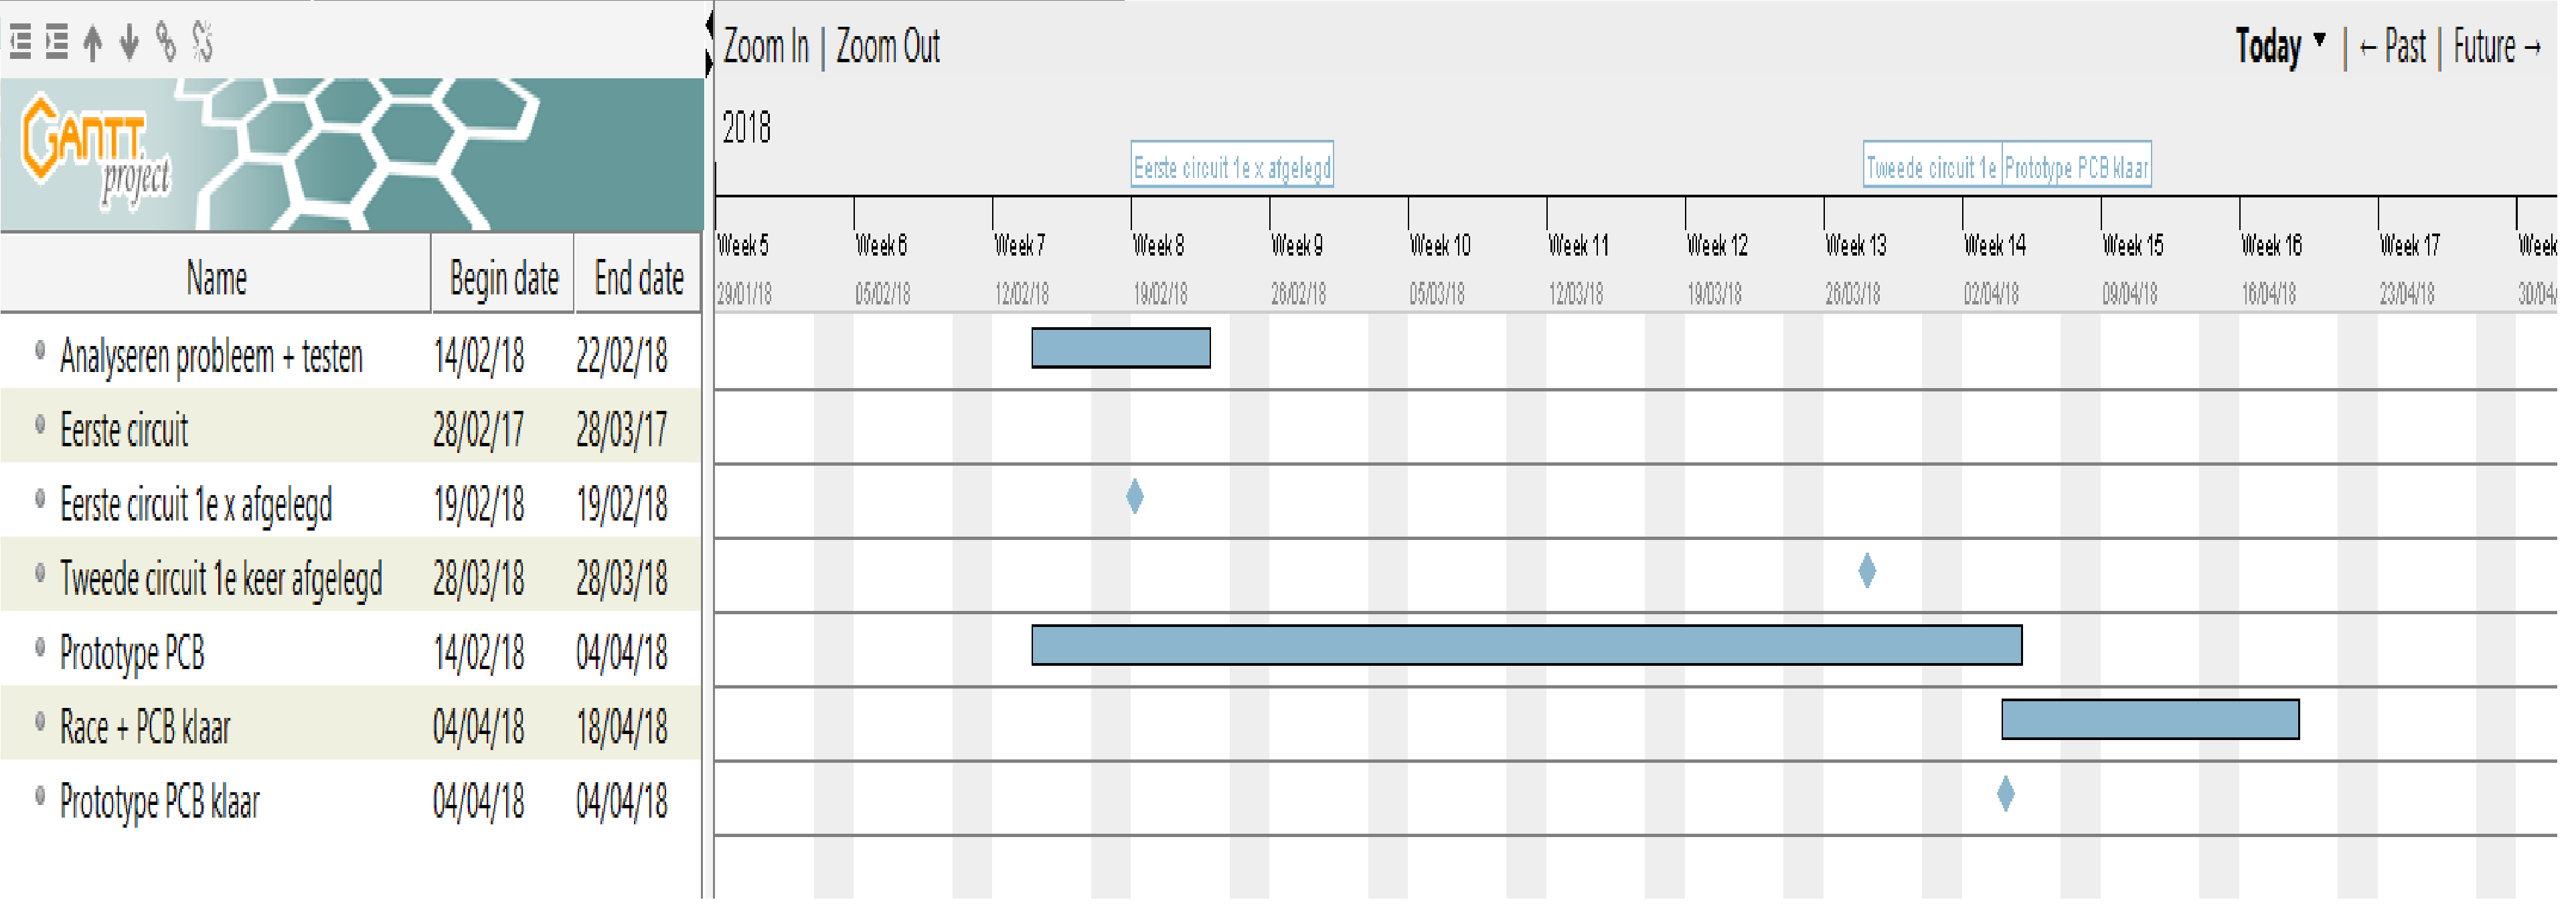
\includegraphics[width=1\textwidth]{planning.png}
\caption{Planning met milestones}
\label{fig:planning}
\end{figure}
